Since all tasks are atomic and have same deadline/period, the scheduling problem reduces to partitioning tasks to HC and LC with the objective of minimizing makespan or minimizing energy consumption. As we will see later in this section, for certain task and system configurations, these two objectives are conflicting. However, in most scenarios, these two objectives lead to the same solution i.e. minimizing makespan also minimizes energy. Formally, we can state the following optimization formulation:
\begin{figure}[h]
\hrulefill\\
\textbf{Variables:}
\begin{equation*}
\alpha_{i,X}=\begin{cases}1,&\mbox{if task ${i}$ is assigned to core $X\in\{\mathrm{HC, LC}\}$ }\\0,&\mbox{otherwise}
\end{cases}
\end{equation*}
\textbf{Objectives:}
\begin{align*}
\text{Obj 1: }& \text{Minimize} \big\{\max\{A_\mathrm{HC}, A_\mathrm{LC}\}\big\}\numberthis\label{equ:obj1}\\
\text{Obj 2: }& \text{Minimize} \big\{P_\mathrm{HC}A_\mathrm{HC}  + P_\mathrm{LC}A_\mathrm{LC} + P_\mathrm{Sys}A_\mathrm{sys}\big\}\numberthis\label{equ:obj2}\\
\text{where: }&A_\mathrm{X}=\sum_{1\leq i\leq n}\frac{\alpha_{i,\mathrm{X}}\cdot C_i}{F_X}\;, X\in\{\mathrm{HC}, \mathrm{LC}\}\\
&A_\mathrm{Sys}=\max\{A_\mathrm{HC}, A_\mathrm{LC} \}  
\end{align*}
\textbf{Constraints:}\\ \vspace{-1em}
\begin{align}
\sum_{X\in\{\mathrm{HC}, \mathrm{LC}\}}\alpha_{i,X}=1\qquad\forall  1\leq i\leq n\\
\max\{A_\mathrm{HC}, A_\mathrm{LC}\}\leq D
\end{align}
\hrulefill
\caption{Mixed Integer Linear Programming (MILP) formulation for the partitioning phase.}
\label{fig:miqcp}
\end{figure}

Objective 1 is minimizing makespan of the application while objective 2 is minimizing the energy consumption during one period $D$. The constraints specify that each task must be assigned to the HC or LC and that the application's makespan must be less than $D$. 

In the following section, we present theoretical results assuming that task-to-core partitioning is fixed/given. Later we will combine these theoretical results with a partitioning heuristic to propose our energy/performance oriented schemes.
Assuming fixed partitioning, we get two \textit{task bins} of possibly different sizes. We denote the total computation cycles of all tasks in the large bin  and small bin by $C_\mathrm{Lg}$ and $C_\mathrm{Sm}$ respectively ($C_\mathrm{Lg}\geq C_\mathrm{Sm}$). We also use an auxiliary variable $\Delta=\frac{C_{\mathrm{Lg}}-C_{\mathrm{Sm}}}{C_{\mathrm{Lg}}+C_{\mathrm{Sm}}}$ to quantify the imbalance between bins. $\Delta=0$ when both bins are equal and it approaches 1 as the imbalance between bins increases. Now we study the characteristics of task partitioning which minimizes makespan/energy. 

\begin{theorem}\label{thm:delta_opt}
The makespan and the energy consumption are simultaneously minimized when $\Delta=\Delta_\mathrm{opt}$, where:
\begin{equation}\label{equ:deltaopt}
\Delta_\mathrm{opt}=\frac{F_\mathrm{HC}-F_\mathrm{LC}}{F_\mathrm{HC}+F_\mathrm{LC}}\;
\end{equation}
 and the large/small task bins are executed in HC/LC respectively.
\end{theorem}
\noindent\textbf{Proof:} When $\Delta=\Delta_\mathrm{opt}$, $\frac{C_\mathrm{HC}-C_\mathrm{LC}}{C_\mathrm{HC}+C_\mathrm{LC}} =\frac{F_\mathrm{HC}-F_\mathrm{LC}}{F_\mathrm{HC}+F_\mathrm{LC}}$. This can be algebraically reduced to $\frac{C_\mathrm{Lg}}{F_\mathrm{Lg}} = \frac{C_\mathrm{Sm}}{F_\mathrm{Sm}}$. L.H.S is $A_\mathrm{HC}$ when HC executes the large task bin and R.H.S is $A_{LC}$ when LC executes the small task bin. Therefore, the active times of both cores are equal. Increasing the computation cycles of LC or HC, by shifting tasks, would increase the corresponding active time; thus increasing makespan. Therefore $\Delta=\Delta_\mathrm{opt}$ leads to the optimal makespan.
Now, we prove that $\Delta=\Delta_\mathrm{opt}$ with HC/LC executing large/small task bins also minimizes energy. Let us suppose that $A^*$ represents the optimal value of makespan. For this value, the energy consumption of the system during one period $D$ is: 
\begin{equation*}
E^*=A^*\cdot (P_\mathrm{HC} + P_\mathrm{LC}+ P_\mathrm{Sys})
\end{equation*}
Now suppose that from this optimal scenario, $0< x\leq A^*\cdot F_\mathrm{LC}$ computation cycles are shifted from the LC to HC. The new energy consumption is:
\begin{equation*}
E_1=(A^*+ \frac{x}{F_\mathrm{HC}})(P_\mathrm{HC} + P_\mathrm{Sys})+ (A^*- \frac{x}{F_\mathrm{LC}})  \cdot P_\mathrm{LC}
\end{equation*} 
Substracting $E^*$ from $E_1$, we get $x/F_\mathrm{HC}\cdot(P_\mathrm{HC}+P_\mathrm{Sys}) - x/F_\mathrm{LC}\cdot P_\mathrm{LC}$; which is always positive due to condition 2. Therefore, $E_1\geq E^*.$ 

Conversely, now suppose that from this optimal scenario, $0< x\leq A^*\cdot F_\mathrm{HC}$ computation cycles are shifted from the HC to LC. The new energy consumption is:
\begin{equation*}
E_2= (A^*- \frac{x}{F_\mathrm{HC}})  \cdot P_\mathrm{HC} +  (A^*+ \frac{x}{F_\mathrm{LC}})(P_\mathrm{LC} + P_\mathrm{Sys}) 
\end{equation*} 
Subtracting $E^*$ from $E_2$, we get $x/F_\mathrm{LC}\cdot(P_\mathrm{LC}+P_\mathrm{Sys}) - x/F_\mathrm{HC}\cdot P_\mathrm{LC}$; which is always positive due to conditions 1 and 3. Therefore, $E_2> E^*$. Consequently, $E^*$ is the minimum possible energy consumption for a given task-set. \qed

%The remaining section studies how tasks should be executed when optimal task partitioning ($\Delta=\Delta_\mathrm{opt}$) cannot be achieved. %when $\Delta\neq\Delta_{\mathrm{opt}}$ and the energy performance tradeoffs thereof. 
%From this point forward, we assume that $\Delta$ (and therefore the partitioning of tasks to bins) is given/fixed. 
Given fixed partitions, we can execute tasks in the following ways:
\begin{enumerate}
\item \textit{Scenario 1}: Large task bin executed on HC and small task bin executed on LC.
\item \textit{Scenario 2}: Small task bin executed on HC and large task bin executed on LC.
\item \textit{Scenario 3}: Both task bins executed on HC. 
\item \textit{Scenario 4}: Both task bins executed on LC. 
\end{enumerate}
We now study the conditions under which these execution scenarios are performance/energy optimal.

\begin{theorem}\label{thm: parallel-perf}
Executing large task bin on HC and small task bin on LC (Scenario 1) is always performance optimal. 
\end{theorem}
\noindent \textbf{Proof:} It is trivial to prove that scenario 1 has lower makespan compared to scenario 2 and scenario 3 has lower makespan compared to scenario 4. We will now prove that Scenario 1 outperforms Scenario 3. i.e. scenario 1 makespan $\leq$ scenario 3 makespan:
\[
\max\{C_\mathrm{Lg}/F_{\mathrm{HC}}, \;C_\mathrm{Sm}/F_{\mathrm{LC}} \}\leq (C_\mathrm{Lg}+C_\mathrm{sm})/F_\mathrm{HC} 
\]
The first term in the $\max$ is always less than RHS. Regarding the second term in the $\max$, $C_\mathrm{Sm}/F_{\mathrm{LC}}\leq $ RHS given condition 1.  \qed


We will now derive conditions for an \textit{energy optimal} scheme. The total energies for the four scenarios are calculated using following equations:  
\begin{align*}
E_{\mathrm{Total},1} =& P_{\mathrm{HC}}\cdot C_\mathrm{Lg}/F_\mathrm{HC} + P_{\mathrm{LC}}  \cdot C_\mathrm{Sm}/F_\mathrm{LC}\\
&+P_{\mathrm{Sys}}\cdot \max(C_\mathrm{Lg}/F_\mathrm{HC},\;C_\mathrm{Sm}/F_\mathrm{LC})\\ 
E_{\mathrm{Total},2} =& P_{\mathrm{HC}}\cdot C_\mathrm{Sm}/F_\mathrm{HC} + (P_{\mathrm{LC}}+ P_{\mathrm{Sys}})  \cdot C_\mathrm{Lg}/F_\mathrm{LC}\\
E_{\mathrm{Total},3} =& (P_{\mathrm{HC}} + P_{\mathrm{Sys}})\cdot (C_\mathrm{Lg}+ C_\mathrm{Sm})/F_\mathrm{HC}\\
E_{\mathrm{Total},4} =& (P_{\mathrm{LC}} + P_{\mathrm{Sys}})\cdot (C_\mathrm{Lg}+ C_\mathrm{Sm})/F_\mathrm{LC}
\end{align*}
\begin{theorem}\label{thm:parallel}
It is always energy optimal to parallelize workload.
\end{theorem}
\noindent\textbf{Proof:} We first prove that $E_\mathrm{Total, 1}\leq E_\mathrm{Total, 3}$. We then prove that $E_\mathrm{Total, 2}\leq E_\mathrm{Total, 4}$, proving that parallelizing workload always leads to lower energy consumption.  
\begin{align*} 
 E_{\mathrm{Total},1}-E_{\mathrm{Total},3}=& P_{\mathrm{LC}} \cdot \frac{C_\mathrm{Sm}}{F_\mathrm{LC}} + P_{\mathrm{Sys}}\cdot \max(\frac{C_\mathrm{Lg}}{F_\mathrm{HC}},\;\frac{C_\mathrm{Sm}}{F_\mathrm{LC}}) 
\\&- P_{\mathrm{HC}} \cdot \frac{C_\mathrm{Sm}}{F_\mathrm{HC}}-P_{\mathrm{Sys}}\cdot \frac{C_\mathrm{Lg}+C_\mathrm{Sm}}{F_\mathrm{HC}}
\end{align*}

By Theorem~\ref{thm: parallel-perf}, $\max\{C_\mathrm{Lg}/F_{\mathrm{HC}}, \;C_\mathrm{Sm}/F_{\mathrm{LC}} \}\leq \frac{C_\mathrm{Lg}+C_\mathrm{sm}}{F_\mathrm{HC}}$. Therefore:
\[ 
 E_{\mathrm{Total},1}-E_{\mathrm{Total},3}\leq P_{\mathrm{LC}} \cdot \frac{C_\mathrm{Sm}}{F_\mathrm{LC}}- P_{\mathrm{HC}} \cdot\frac{C_\mathrm{Sm}}{F_\mathrm{HC}}
\]
R.H.S is always $\leq 0$ due to condition 2, therefore $E_\mathrm{Total, 1}\leq E_\mathrm{Total, 3}$. We now prove $E_\mathrm{Total,2}\leq E_\mathrm{Total,4}$:
\begin{equation*}
\begin{split}
E_\mathrm{Total,2}-E_\mathrm{Total,4}=P_{\mathrm{HC}}\cdot \frac{C_\mathrm{Sm}}{F_\mathrm{HC}} - (P_{\mathrm{LC}}+P_{\mathrm{Sys}})  \cdot \frac{C_\mathrm{Sm}}{F_\mathrm{LC}} 
\end{split}
\end{equation*}
R.H.S. $\leq$ 0 if conditions 1 and 3 are valid. \qed

We now derive conditions where the scenario 1 and scenario 2 are energy optimal. 

%Note that for scenario 2, $P_{\mathrm{sys},A}$ is consumed for $A_{\mathrm{LC},2}$ because $A_{\mathrm{LC},2}\geq A_{\mathrm{HC},2}$ irrespective of the value of $\Delta$.
\begin{theorem}\label{thm:case1vscase2}
$E_{\mathrm{Total},1}\leq E_{\mathrm{Total},2}$ \textbf{iff}: $\Delta\leq\max\{\Delta_\mathrm{opt},\; \Delta_\mathrm{diff}\}$, where:
\begin{equation}\label{equ:deltadiff}
\Delta_\mathrm{diff}=\frac{P_\mathrm{Sys} (F_\mathrm{HC}-F_\mathrm{LC})}{2 (F_\mathrm{LC}  P_\mathrm{HC} - F_\mathrm{HC} P_\mathrm{LC}) - P_\mathrm{Sys} (F_\mathrm{HC}-F_\mathrm{LC})} 
\end{equation}
\end{theorem}
\noindent\textbf{Proof:} We prove this for two cases: $\Delta\leq\Delta_\mathrm{opt}$ and $\Delta>\Delta_\mathrm{opt}$.\\
\textbf{Case 1:} $0\leq\Delta\leq \Delta_\mathrm{opt}$. In Scenario 1, $A_\mathrm{HC}\leq A_\mathrm{LC}$. Therefore, the active time of the system $A_\mathrm{Sys}=A_\mathrm{LC}=C_\mathrm{Sm}/F_\mathrm{LC}$. So:
\begin{align*}
E_\mathrm{Total, 1}-E_\mathrm{Total, 2}=&P_\mathrm{HC}(C_\mathrm{Lg}-C_\mathrm{Sm})/F_\mathrm{HC} \\& -(P_\mathrm{LC}+P_\mathrm{Sys})(C_\mathrm{Lg}-C_\mathrm{Sm})/F_\mathrm{LC}
\end{align*}
The positive term in this equation is never greater than the negative term due to conditions 1 and 3. Therefore $E_\mathrm{Total, 1}\leq E_\mathrm{Total, 2}\; \forall \; 0\leq\Delta\leq \Delta_\mathrm{opt}$. \\
\textbf{Case 2:} $\Delta> \Delta_\mathrm{opt}$. In Scenario 1, $A_\mathrm{HC}>A_\mathrm{LC}$. Therefore, the active time of the system $A_\mathrm{Sys}=A_\mathrm{HC}=C_\mathrm{Lg}/F_\mathrm{HC}$. We now find the condition where $E_\mathrm{Total, 1}-E_\mathrm{Total, 2}\leq 0$
\begin{align*}
P_\mathrm{HC}(C_\mathrm{Lg}-C_\mathrm{Sm})/F_\mathrm{HC} - P_\mathrm{LC}(C_\mathrm{Lg}-C_\mathrm{Sm})/F_\mathrm{LC}\\
-P_\mathrm{Sys}\cdot C_\mathrm{Lg}(F_\mathrm{HC}-F_\mathrm{LC})/(F_\mathrm{HC}\cdot F_\mathrm{LC})&\leq 0\\ 
\implies \frac{P_\mathrm{HC}}{F_\mathrm{HC}}-\frac{P_\mathrm{LC}}{F_\mathrm{LC}}-P_\mathrm{Sys}\frac{C_\mathrm{Lg}}{{C_\mathrm{Lg}-C_\mathrm{Sm}}}\frac{F_\mathrm{HC}-F_\mathrm{LC}}{F_\mathrm{HC}\cdot F_\mathrm{LC}}&\leq 0
\end{align*}
Substituting $\frac{C_\mathrm{Lg}}{{C_\mathrm{Lg}-C_\mathrm{Sm}}} = \frac{\Delta+1}{2\Delta}$ and solving to $\Delta$ leads to the R.H.S of \eqref{equ:deltadiff}. Combining case 1 and case 2 conditions proves the theorem.\qed

\subsection{Task Allocation Policies}
Firstly, all tasks are partitioned with the objective of making $\Delta=\Delta_\mathrm{opt}=\frac{F_\mathrm{HC}-F_\mathrm{LC}}{F_\mathrm{HC}+F_\mathrm{LC}}$. We utilize a heuristic algorithm that does bin-packing of tasks to cores with the objective of $\Delta=\Delta_\mathrm{opt}$. Specifically, given a set of tasks and two uniform (non-identical) cores, assign tasks to cores such that makespan is minimized. This is a well studied $Q2||C_{\mathrm{max}}$ problem and is known to be NP-Hard. However, the Modified Longest Processing Time (MLPT) heuristic proposed in \cite{mlpt} solves this problem with an approximation ratio of 1.22. MLPT also has low complexity $O(n\log n +c)$ and therefore can be applied at runtime. The working of MLPT algorithm is summarized here for completeness:
\begin{enumerate}
	\item Sort all tasks in non-increasing order of their computation times.
	\item if $n\leq2$, assign tasks greedily such that their individual completion/finish time is minimized. 
	\item if $n\geq 3$, assign the first three (largest) tasks optimally such that their makespan is minimized. Assign the remaining tasks greedily such that their individual completion/finish time is minimized.
\end{enumerate}
Next, the task bins are executed using the following policies:
\begin{enumerate}
\item \emph{Delta Threshold Mapping-Makespan (DTM-M)}: Execute \textit{Large} task bin on the HC and \textit{Small} task bin on LC.
\item \emph{Delta Threshold Mapping-Energy (DTM-E)}: Execute \textit{Large} task bin on HC and \textit{Small} task bin on the LC if $\Delta \leq \max\{\Delta_\mathrm{opt},\;\Delta_\mathrm{diff}\}$ \textbf{OR} $\frac{C_\mathrm{Lg}}{F_\mathrm{LC}}\leq D$. %$\Delta_\mathrm{opt}$ and $\Delta_\mathrm{diff}$ are defined in equations \eqref{equ:deltaopt} and \eqref{equ:deltadiff} respectively. 
Do the converse otherwise. 
\end{enumerate}
The optimality of these approaches for a given partitioning has been proved in Theorem \ref{thm: parallel-perf} and \ref{thm:case1vscase2}. 

\begin{figure*}[!t]
	\centering
	\begin{subfigure}{.5\columnwidth}
		\centering
		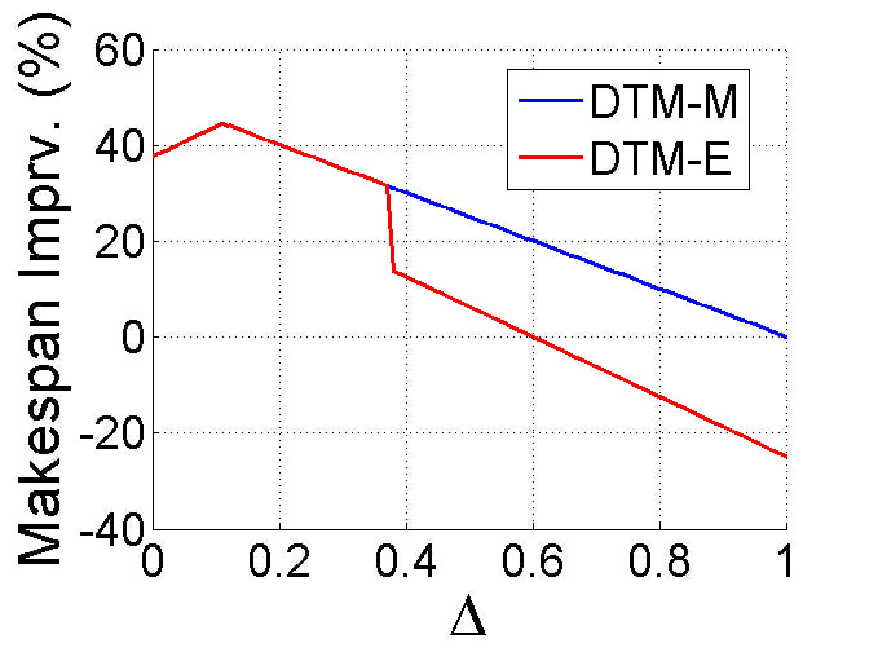
\includegraphics[width=\columnwidth]{./figures/flc_80_delta_makespan_theory}
		\caption{Makespan Simulation}
		\label{fig:Flc80-delta-makespan-theory}
	\end{subfigure}
	\begin{subfigure}{.5\columnwidth}
		\centering
		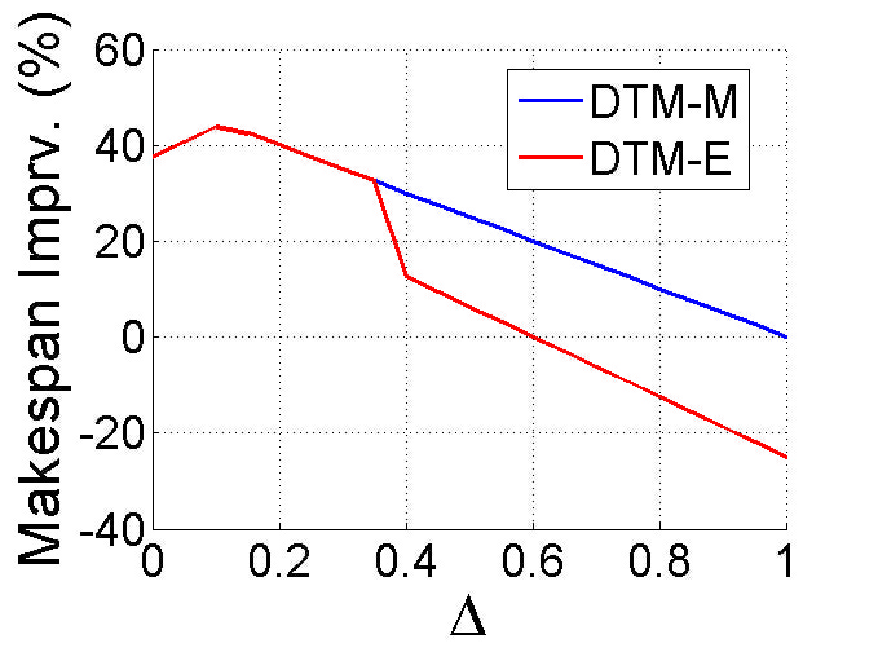
\includegraphics[width=\columnwidth]{./figures/flc_80_delta_makespan}
		\caption{Makespan Experiment}
		\label{fig:Flc80-delta-makespan}
	\end{subfigure}
	\begin{subfigure}{.5\columnwidth}
		\centering
		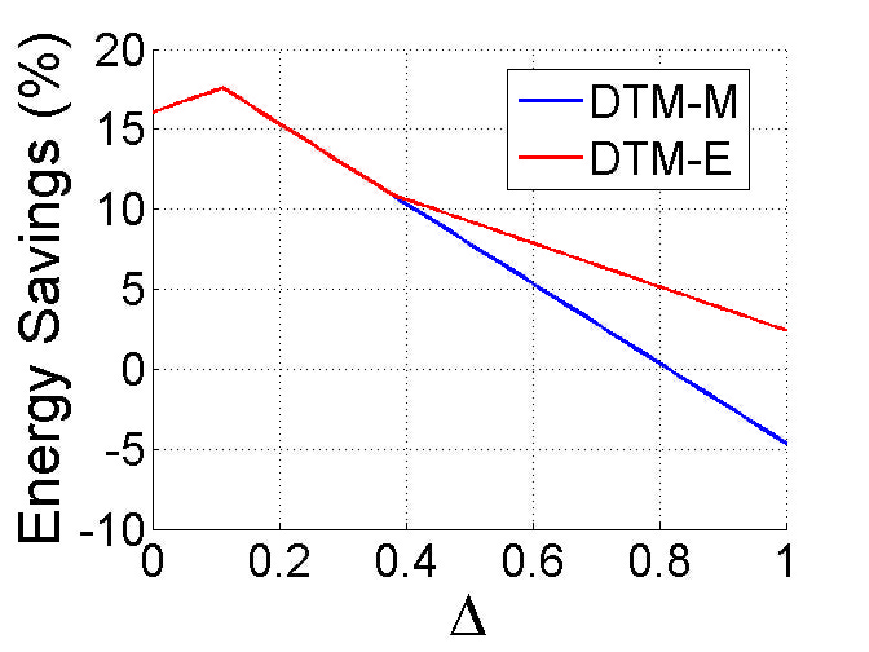
\includegraphics[width=\columnwidth]{./figures/flc_80_delta_energy_theory}
		\caption{Energy Simulation}
		\label{fig:Flc80-delta-energy-theory}
	\end{subfigure}
	\begin{subfigure}{.5\columnwidth}
		\centering
		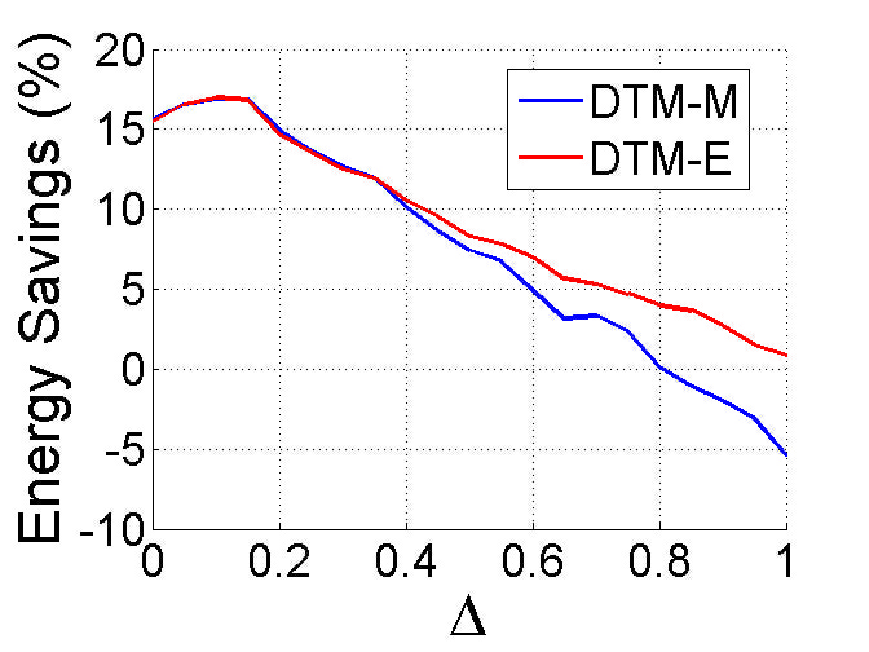
\includegraphics[width=\columnwidth]{./figures/flc_80_delta_energy}
		\caption{Energy Experiment}
		\label{fig:Flc80-delta-energy}
	\end{subfigure}
	\caption{Dynamic Threshold Mapping (DTM) Energy and Performance Results for $F_{LC} = 80 MHz$ and utilization = 50\%.}
	\label{fig:Flc80-delta}
\end{figure*}